% TikZ test snippet for Q6 (椭圆和直线)
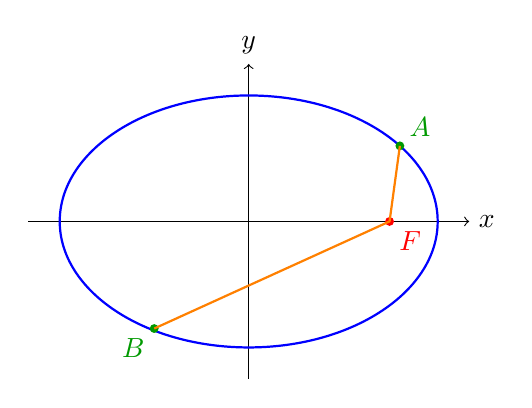
\begin{tikzpicture}[scale=0.8]
  % 坐标轴
  \draw[->] (-3.5,0) -- (3.5,0) node[right] {$x$};
  \draw[->] (0,-2.5) -- (0,2.5) node[above] {$y$};
  
  % 椭圆
  \draw[thick,blue] (0,0) ellipse (3 and 2);
  
  % 焦点 F
  \fill[red] ({sqrt(5)},0) circle (2pt) node[below right] {$F$};
  
  % 点 A 和 B
  \fill[green!60!black] (2.4,1.2) circle (2pt) node[above right] {$A$};
  \fill[green!60!black] (-1.5,-1.7) circle (2pt) node[below left] {$B$};
  
  % 直线 BF
  \draw[thick,orange] (-1.5,-1.7) -- ({sqrt(5)},0) -- (2.4,1.2);
\end{tikzpicture}
